\chapter*{Introduction Générale}
\addcontentsline{toc}{chapter}{Introduction Générale}

\section*{Le Cadre du Concours de Recrutement}
Le concours d'accès au grade d'\textbf{Ingénieur d'État de premier grade} au sein du \textbf{Ministère des Affaires Étrangères, de la Coopération Africaine et des Marocains Résidant à l'Étranger (MAECAME)} est organisé par la Direction des Affaires Administratives et Générales du ministère, dans le cadre du statut du corps interministériel des ingénieurs et architectes (décret n° 2-05-1367) et du statut particulier du personnel du ministère (décret n° 2-04-534). L'avis de la session 2026 (code C43032/26) ouvre \textbf{16 postes} à l'échelle 11 : \textbf{10 en Réseaux et Télécommunications} et \textbf{6 en Développement informatique}, dont un poste réservé au secteur des Marocains résidant à l'étranger. La sélection est exigeante : \textbf{1 472 candidats} ont été convoqués aux épreuves écrites du 27 septembre 2026, soit environ un poste pour 92 candidats. Lors de la session précédente (23 novembre 2025, 17 postes), environ 943 candidats avaient été convoqués, 149 admis à l'oral et 17 recrutés.

Le ministère n'est pas une administration comme les autres : il porte la voix du Royaume dans le monde, défend son intégrité territoriale, anime sa coopération avec l'Afrique et accompagne plus de cinq millions de Marocains du monde à travers un réseau d'environ 104 ambassades et missions permanentes et 53 consulats généraux répartis sur tous les fuseaux horaires.

\section*{Pourquoi le Ministère recrute-t-il des Ingénieurs d'État ?}
Une diplomatie moderne repose sur des systèmes d'information sûrs, disponibles en permanence et accessibles depuis le monde entier :
\begin{itemize}
    \item \textbf{Réseaux et télécommunications :} interconnexion sécurisée de plus de 150 postes à l'étranger avec l'administration centrale (VPN, liaisons chiffrées, redondance, communications diplomatiques), téléphonie et visioconférence, continuité de service.
    \item \textbf{Services consulaires numériques :} plateformes \texttt{consulat.ma} et \texttt{rdv.consulat.ma}, système interne eConsulat, e-Visa (\texttt{acces-maroc.ma}, lancé en juillet 2022), apostille électronique, état civil consulaire et échanges avec les administrations nationales (Intérieur, Justice, Registre National de la Population).
    \item \textbf{Cybersécurité et protection des données :} le ministère traite des informations sensibles (correspondance diplomatique, données personnelles des Marocains du monde et des demandeurs de visa) soumises à la loi 05-20 sur la cybersécurité, à la Directive Nationale de la Sécurité des Systèmes d'Information (DNSSI) de la DGSSI et à la loi 09-08 sur les données personnelles.
    \item \textbf{Direction des Systèmes d'Information :} créée par le décret n° 2.24.957 du 21 novembre 2024 au sein de la Direction Générale des Affaires Administratives et Générales, elle élabore et exécute les plans du ministère en matière de systèmes d'information, gère l'infrastructure et garantit la cybersécurité.
    \item \textbf{Diplomatie de la donnée et de l'image :} veille et analyse de l'information, communication numérique, tableaux de bord au service de la diplomatie économique et de la mobilisation des compétences des Marocains du monde.
\end{itemize}

\IfFileExists{images/img_001_intro_ecosysteme_si_maecame.png}{%
\begin{figure}[H]
    \centering
    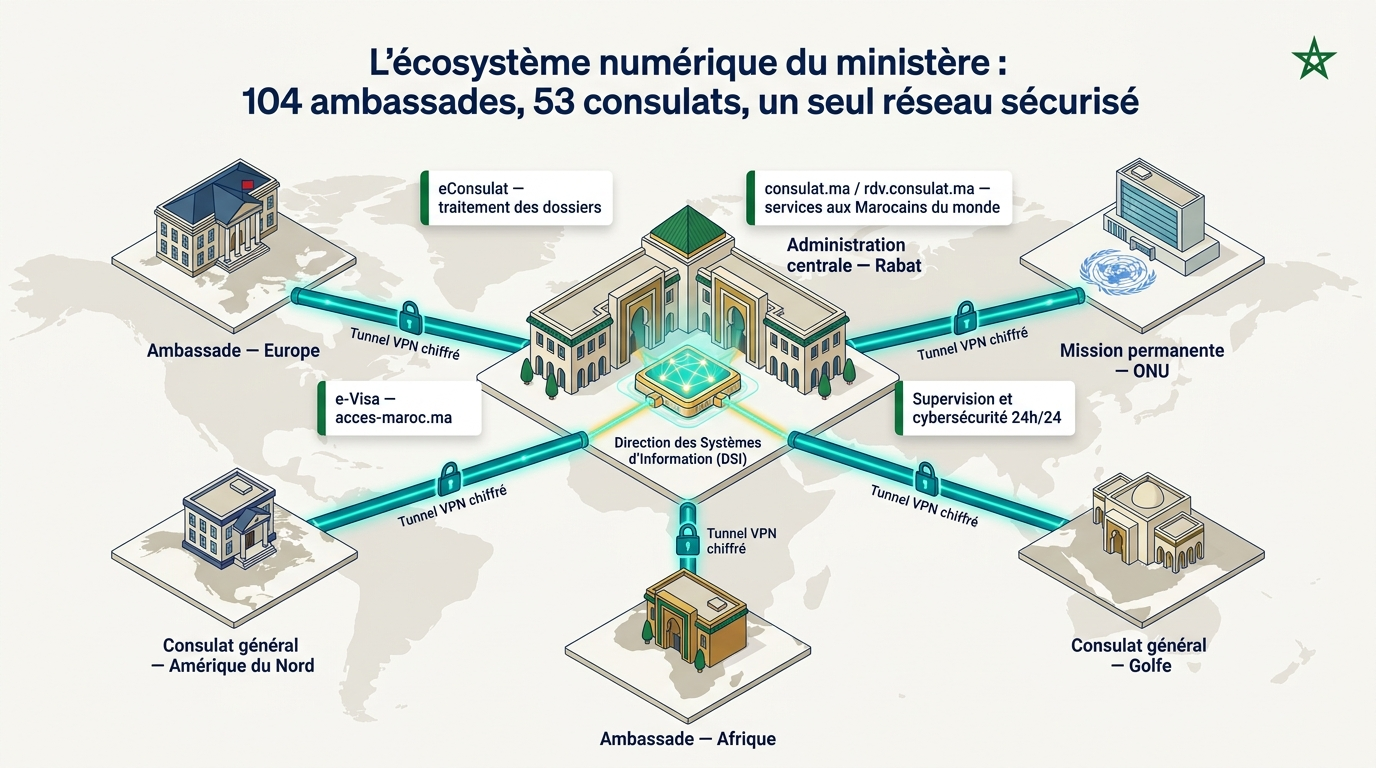
\includegraphics[width=\textwidth]{images/img_001_intro_ecosysteme_si_maecame.png}
    \caption*{\textbf{Illustration introductive :} L'écosystème numérique du MAECAME, de l'administration centrale au réseau diplomatique et consulaire}
\end{figure}}{}

Le jury attend donc un \textbf{ingénieur solide techniquement} (l'épreuve de spécialité compte pour un tiers de la note finale, et l'oral, largement technique, pour la moitié), mais aussi un \textbf{cadre de l'État capable de comprendre les missions du ministère} et d'inscrire ses solutions dans les priorités de la diplomatie marocaine.

\section*{Les Trois Épreuves et leur Poids}
\begin{table}[H]
\centering
\small
\begin{tabular}{|p{5.2cm}|c|c|c|p{4.6cm}|}
\hline
\rowcolor{gray!20} \textbf{Épreuve} & \textbf{Durée} & \textbf{Coef.} & \textbf{Poids} & \textbf{Contenu (avis officiel)} \\ \hline
Écrit (a) : Spécialité & 3 h & 4 & 33 \% & Spécialité(s) demandée(s), fonctions ou postes à occuper en informatique et en réseaux. \\ \hline
Écrit (b) : Rédaction & 2 h & 2 & 17 \% & Rédaction d'un sujet portant sur les attributions du ministère. \\ \hline
Oral : Entretien & 30-40 min & 6 & 50 \% & Discussion avec le jury de sujets et questions variés pour évaluer l'aptitude à exercer les fonctions. \\ \hline
\end{tabular}
\caption{Barème du concours 2026 (avis officiel C43032/26)}
\end{table}

\IfFileExists{images/img_011_bareme_trois_epreuves.png}{%
\begin{figure}[H]
    \centering
    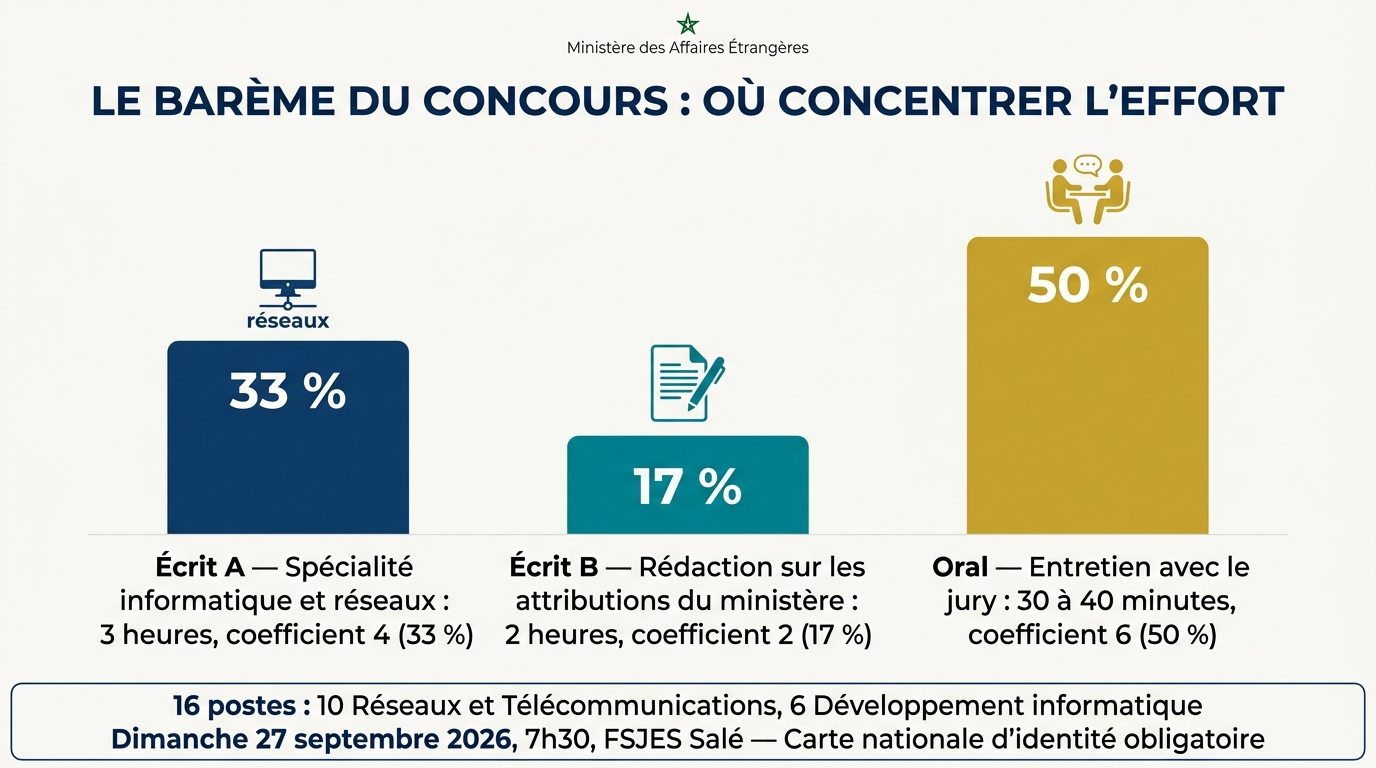
\includegraphics[width=\textwidth]{images/img_011_bareme_trois_epreuves.png}
    \caption*{Le barème du concours : où concentrer l'effort}
\end{figure}}{}

L'avis ne précise ni la forme exacte de l'épreuve de spécialité (QCM, questions ouvertes ou exercices), ni la langue, ni un seuil d'admissibilité : il faut se préparer à toutes les formes et savoir rédiger en français comme en arabe pour les notions institutionnelles.

\section*{Objectif et Organisation du Présent Guide}
Face à une échéance à quatre jours, ce guide vise l'efficacité immédiate :
\begin{enumerate}
    \item \textbf{Comprendre ce qui est réellement noté :} les trois épreuves, leur poids et les attentes d'un jury de diplomates et d'ingénieurs.
    \item \textbf{Maîtriser la matière diplomatique :} organisation du ministère, constantes de la politique étrangère, Sahara, Afrique, Marocains du monde, partenariats, avec des sujets de rédaction entièrement traités.
    \item \textbf{Réussir l'épreuve de spécialité :} réseaux et télécommunications, développement et bases de données, cybersécurité, avec exercices corrigés adaptés au contexte du ministère.
    \item \textbf{S'entraîner en conditions réelles :} planning J-4 et examen blanc complet avec corrigés.
\end{enumerate}
